%File: anonymous-submission-latex-2024.tex
\documentclass[letterpaper]{article} % DO NOT CHANGE THIS
\usepackage{aaai24}  % DO NOT CHANGE THIS
\usepackage{times}  % DO NOT CHANGE THIS
\usepackage{helvet}  % DO NOT CHANGE THIS
\usepackage{courier}  % DO NOT CHANGE THIS
\usepackage[hyphens]{url}  % DO NOT CHANGE THIS
\usepackage{booktabs}
\usepackage{graphicx} % DO NOT CHANGE THIS
\usepackage{multicol}

% \usepackage[margin=1in]{geometry}

\urlstyle{rm} % DO NOT CHANGE THIS
\def\UrlFont{\rm}  % DO NOT CHANGE THIS
\usepackage{natbib}  % DO NOT CHANGE THIS AND DO NOT ADD ANY OPTIONS TO IT
\usepackage{caption} % DO NOT CHANGE THIS AND DO NOT ADD ANY OPTIONS TO IT
\frenchspacing  % DO NOT CHANGE THIS
\setlength{\pdfpagewidth}{8.5in} % DO NOT CHANGE THIS
\setlength{\pdfpageheight}{11in} % DO NOT CHANGE THIS
%
% These are recommended to typeset algorithms but not required. See the subsubsection on algorithms. Remove them if you don't have algorithms in your paper.
\usepackage{algorithm}
\usepackage{algorithmic}

%
% These are are recommended to typeset listings but not required. See the subsubsection on listing. Remove this block if you don't have listings in your paper.
\usepackage{newfloat}
\usepackage{listings}
\DeclareCaptionStyle{ruled}{labelfont=normalfont,labelsep=colon,strut=off} % DO NOT CHANGE THIS
\lstset{%
	basicstyle={\footnotesize\ttfamily},% footnotesize acceptable for monospace
	numbers=left,numberstyle=\footnotesize,xleftmargin=2em,% show line numbers, remove this entire line if you don't want the numbers.
	aboveskip=0pt,belowskip=0pt,%
	showstringspaces=false,tabsize=2,breaklines=true}
\floatstyle{ruled}
\newfloat{listing}{tb}{lst}{}
\floatname{listing}{Listing}
%
% Keep the \pdfinfo as shown here. There's no need
% for you to add the /Title and /Author tags.
\pdfinfo{
/TemplateVersion (2024.1)
}


\usepackage{listings}
\usepackage{xcolor}

\definecolor{codegreen}{rgb}{0,0.6,0}
\definecolor{codegray}{rgb}{0.5,0.5,0.5}
\definecolor{codepurple}{rgb}{0.58,0,0.82}
\definecolor{backcolour}{rgb}{0.95,0.95,0.92}

\lstdefinestyle{mystyle}{
    backgroundcolor=\color{backcolour},   
    commentstyle=\color{codegreen},
    keywordstyle=\color{magenta},
    numberstyle=\tiny\color{codegray},
    stringstyle=\color{codepurple},
    basicstyle=\footnotesize\ttfamily,
    breakatwhitespace=false,         
    breaklines=true,                 
    captionpos=b,                    
    keepspaces=true,                 
    numbers=left,                    
    numbersep=5pt,                  
    showspaces=false,                
    showstringspaces=false,
    showtabs=false,                  
    tabsize=2
}

\lstset{style=mystyle}


% DISALLOWED PACKAGES
% \usepackage{authblk} -- This package is specifically forbidden
% \usepackage{balance} -- This package is specifically forbidden
% \usepackage{color (if used in text)
% \usepackage{CJK} -- This package is specifically forbidden
% \usepackage{float} -- This package is specifically forbidden
% \usepackage{flushend} -- This package is specifically forbidden
% \usepackage{fontenc} -- This package is specifically forbidden
% \usepackage{fullpage} -- This package is specifically forbidden
% \usepackage{geometry} -- This package is specifically forbidden
% \usepackage{grffile} -- This package is specifically forbidden
% \usepackage{hyperref} -- This package is specifically forbidden
% \usepackage{navigator} -- This package is specifically forbidden
% (or any other package that embeds links such as navigator or hyperref)
% \indentfirst} -- This package is specifically forbidden
% \layout} -- This package is specifically forbidden
% \multicol} -- This package is specifically forbidden
% \nameref} -- This package is specifically forbidden
% \usepackage{savetrees} -- This package is specifically forbidden
% \usepackage{setspace} -- This package is specifically forbidden
% \usepackage{stfloats} -- This package is specifically forbidden
% \usepackage{tabu} -- This package is specifically forbidden
% \usepackage{titlesec} -- This package is specifically forbidden
% \usepackage{tocbibind} -- This package is specifically forbidden
% \usepackage{ulem} -- This package is specifically forbidden
% \usepackage{wrapfig} -- This package is specifically forbidden
% DISALLOWED COMMANDS
% \nocopyright -- Your paper will not be published if you use this command
% \addtolength -- This command may not be used
% \balance -- This command may not be used
% \baselinestretch -- Your paper will not be published if you use this command
% \clearpage -- No page breaks of any kind may be used for the final version of your paper
% \columnsep -- This command may not be used
% \newpage -- No page breaks of any kind may be used for the final version of your paper
% \pagebreak -- No page breaks of any kind may be used for the final version of your paperr
% \pagestyle -- This command may not be used
% \tiny -- This is not an acceptable font size.
% \vspace{- -- No negative value may be used in proximity of a caption, figure, table, section, subsection, subsubsection, or reference
% \vskip{- -- No negative value may be used to alter spacing above or below a caption, figure, table, section, subsection, subsubsection, or reference

\setcounter{secnumdepth}{0} %May be changed to 1 or 2 if section numbers are desired.

% The file aaai24.sty is the style file for AAAI Press
% proceedings, working notes, and technical reports.
%

% Title

% Your title must be in mixed case, not sentence case.
% That means all verbs (including short verbs like be, is, using,and go),
% nouns, adverbs, adjectives should be capitalized, including both words in hyphenated terms, while
% articles, conjunctions, and prepositions are lower case unless they
% directly follow a colon or long dash
\title{Supplementary Methods}
% \author{
%     %Authors
%     % All authors must be in the same font size and format.
%     Jaeff Hong\equalcontrib\textsuperscript{\rm 2}, Duong Dung\equalcontrib\textsuperscript{\rm 1}, Dani Hutchison\textsuperscript{\rm 1}, Zubair Akhtar\textsuperscript{\rm 1}, Rosalie Chen\textsuperscript{\rm 1}, Rebecca Dawson\textsuperscript{\rm 1}, Aditya Joshi\textsuperscript{\rm 2}, Samsung Lim\textsuperscript{\rm 1}, C Raina MacIntyre\textsuperscript{\rm 1} and Deepti Gurdasani\textsuperscript{\rm 1 \rm 3 \rm 4}, \\
% }
% \affiliations{
%     %Afiliations
%     \textsuperscript{\rm 1}Kirby Institute, University of New South Wales, Sydney, Australia\\
%     % If you have multiple authors and multiple affiliations
%     % use superscripts in text and roman font to identify them.
%     % For example,
%  \textsuperscript{\rm 2}School of Computer Science \& Engineering, University of New South Wales, Sydney, Australia\\
%  \textsuperscript{\rm 3}William Harvey Research Institute, Queen Mary University of London, London, UK\\
%  \textsuperscript{\rm 4}School of Medicine, University of Western Australia, WA, Australia\\

% }

%Example, Single Author, ->> remove \iffalse,\fi and place them surrounding AAAI title to use it
\iffalse
\title{My Publication Title --- Single Author}
\author {
    Author Name
}
\affiliations{
    Affiliation\\
    Affiliation Line 2\\
    name@example.com
}
\fi

\iffalse
%Example, Multiple Authors, ->> remove \iffalse,\fi and place them surrounding AAAI title to use it
\title{My Publication Title --- Multiple Authors}
\author {
    % Authors
    First Author Name\textsuperscript{\rm 1},
    Second Author Name\textsuperscript{\rm 2},
    Third Author Name\textsuperscript{\rm 1}
}
\affiliations {
    % Affiliations
    \textsuperscript{\rm 1}Affiliation 1\\
    \textsuperscript{\rm 2}Affiliation 2\\
    firstAuthor@affiliation1.com, secondAuthor@affilation2.com, thirdAuthor@affiliation1.com
}
\fi


% REMOVE THIS: bibentry
% This is only needed to show inline citations in the guidelines document. You should not need it and can safely delete it.
\usepackage{bibentry}
% END REMOVE bibentry

\begin{document}

\maketitle


\section{Prompt used to generate synthetic data}

We used the following prompt in GPT3.5 to generate synthetic data:

\textbf{System instruction:} 
\begin{lstlisting}
You are an AI content creator who helps to write news about epidemic around the world.
\end{lstlisting}

\textbf{User instruction}:  
\begin{lstlisting}
I have an example articles:
Example:
Title: Ebola Virus Epidemic: 25 new cases reported in Democratic Republic of Congo
Publication date: October 5, 2021

Content: The Ebola virus epidemic in the Democratic Republic of Congo has shown a recent surge in new cases. According to the World Health Organization, 25 new cases were reported in the past week, bringing the total number of cases to 3,825, with 2,589 deaths. The outbreak, which began in August 2018, is the second deadliest in history, after the 2014-2016 West Africa epidemic that killed more than 11,000 people. The WHO and its partners are continuing to work on the ground to control the spread of the virus, including through vaccination campaigns and community engagement. However, the ongoing conflict in the region and resistance from some communities have made the response more challenging.

Please help me to create another one. 
\end{lstlisting}


\section{Prompt used to generate entity and relation triplets for synthetic data}

In designing our prompt to identify entities and relations we aimed to be as specific and simple as possible. The prompt engineering was tailored towards striking a balance between specificity and simplicity where we found by including the list of entities of relations in the prompt, the models could better understand the task at hand and generate responses that aligned closely with expectations. We used the following prompt in GPT3.5 to extract entities and relationships within synthetic data generated using GPT3.5:

\textbf{System instruction:} 
\begin{lstlisting}
You are a smart and intelligent Relation Extraction (RE) system for diseases information.
\end{lstlisting}


% \begin{figure*}[h]
% \centering
% 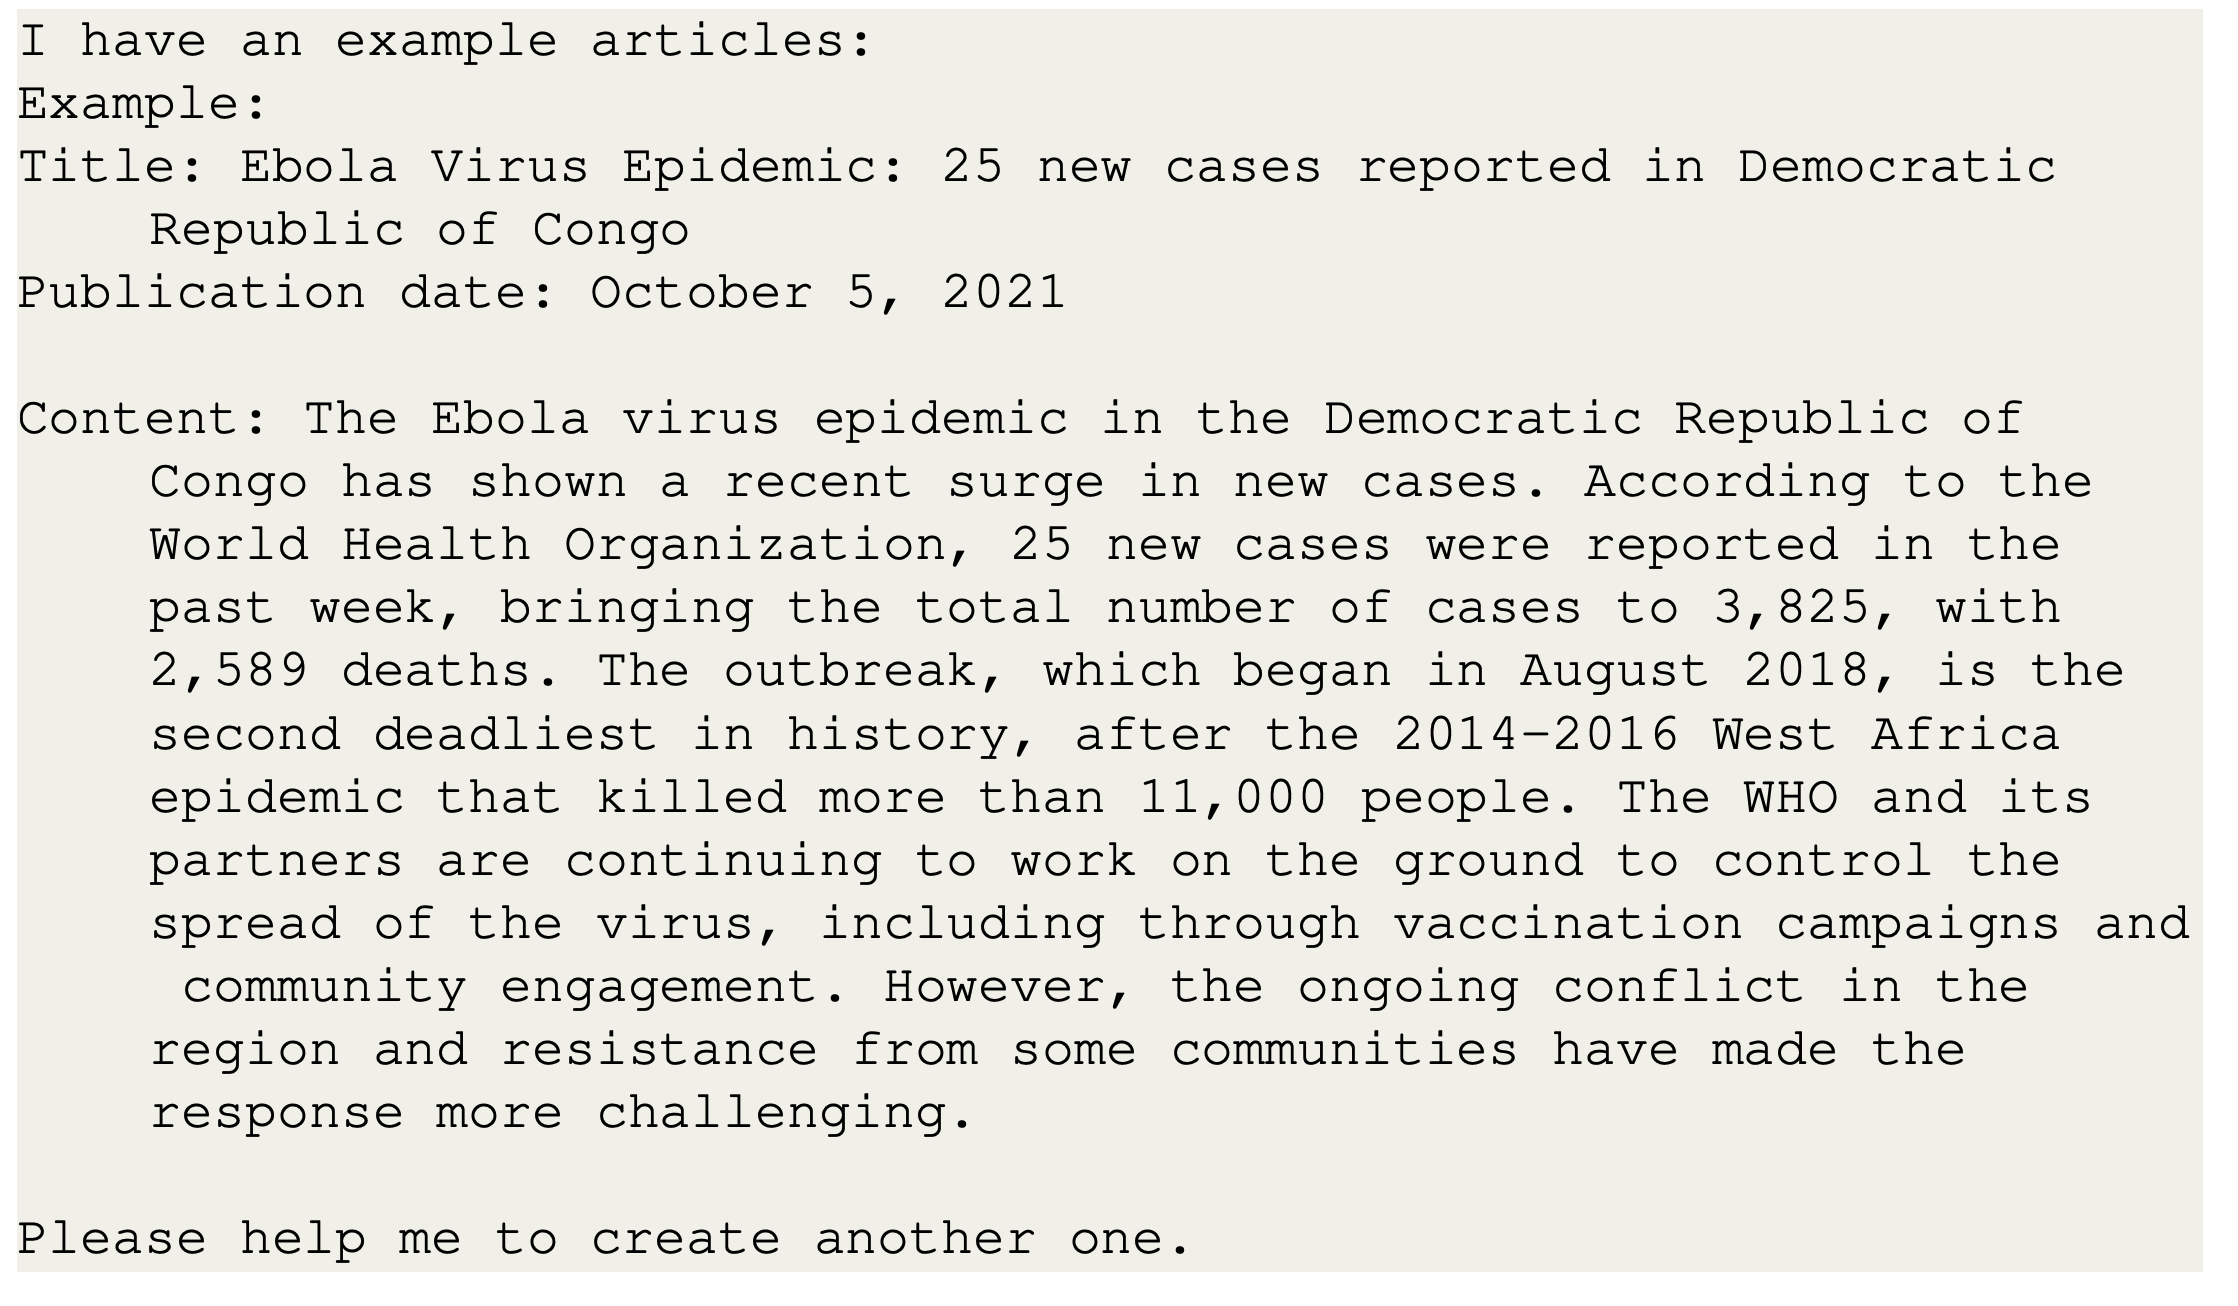
\includegraphics[width=1\textwidth, height=0.4\textheight]{figs/prompt1.png}
% \caption{Architecture}
% \label{fig1}
% \end{figure*}

\textbf{User instruction}:  

\begin{lstlisting}
  I have the list of relations including:
- "located at" is between: disease - location, symptom/syndrome - location, case number - location
- "occurred on" is between: disease - date, symptom/syndrome - date, case number - date
- "are symptoms of" is between: disease - symptom/syndrome
- "deaths of" is between: disease - death numbers
- "cases of" is between: disease - case numbers, symptom/syndrome - case numbers
- "caused by" is between: disease - pathogen
- "affected by" is between: people - disease
Extract all relations between infectious disease, pathogen, symptoms, syndromes, case numbers, date and location from the main body of the article.                   
Example:
Article: Laos reports two H5N1 avian influenza poultry outbreaks, WHO follow-up on human case - Outbreak News Today Follow Privacy Policy US News Europe Asia Africa Latin America and the Caribbean Canada Indian subcontinent Australia Middle East BREAKING Poland reports 12 trichinosis in first half of 2023 Virginia Tech researchers to study lingering Lyme disease symptoms, Awarded NIH grant Malawi cholera update Denmark reports increase in pertussis cases in May and June 2023 Dominican Republic: 11 cases of acute diarrhea, suspected of cholera Outbreak News Radio Interviews Drugs and antibiotics Vaccines Research Blogs TRENDING US News Latin America and the Caribbean Animal diseases Home Asia Laos reports two H5N1 avian influenza poultry outbreaks, WHO follow-up on human case Laos reports two H5N1 avian influenza poultry outbreaks, WHO follow-up on human case by News Desk November 19, 2020 Asia, Headlines No Comments By NewsDesk @ bactiman63 Poultry outbreaks Last Saturday, Dr Vilayphone Vorraphim, Director General of the Department of Livestock and Fisheries with the Ministry of Agriculture and Forestry in Vientiane, Laos reported two Highly pathogenic avian influenza (HPAI) virus (H5N1) outbreaks in two villages in Saravane province. The report to the the World Organisation for Animal Health (OIE) noted that the two outbreaks occurred in the villages of Khantharath and Nakhoysao. More than 500 birds died in the two villages due to the virus. The case is a one-year-old female who developed symptoms of fever, productive cough, difficulty breathing and runny nose on 13 October 2020. She was hospitalized for her illness on 16 October and discharged on 19 October. As part of severe acute respiratory infection (SARI) sentinel surveillance, a specimen was collected on the date of hospitalization and confirmed to be positive for avian influenza A (H5N1) on 28 October by reverse transcription polymerase chain reaction (RT-PCR) at the National Centre for Laboratory and Epidemiology (NCLE).
\end{lstlisting}
            

\textbf{Output:}
\begin{lstlisting}
1) "infectious disease": "avian influenza (HPAI) virus (H5N1)", "relation": "located at", "location": "Saravane province"
2) "infectious disease": "avian influenza (HPAI) virus (H5N1)", "relation": "located at", "location": "Khantharath"
3) "syndrome": "fever, productive cough, difficulty breathing and runny nose", "relation": "occurred on", "event date": "13 October 2020"
4) "overall confirmed deaths": "500", "relation": "deaths of", "host": "one-year-old female"
5) "new confirmed cases": "two", "relation": "cases of", "infectious disease": "avian influenza (HPAI) virus (H5N1)"
Article: {content}
Output:
"""
\end{lstlisting}


\section{Configuration Hyperparameters}


% \begin{lstlisting}
\begin{itemize}
    \item model\_type: LlamaForCausalLM
    \item tokenizer\_type: LlamaTokenizer
    \item is\_llama\_derived\_model: true
    \item load\_in\_8bit: false
    \item load\_in\_4bit: true
    \item strict: false
    \item val\_set\_size: 0.01
    \item adapter: qlora
    \item sequence\_len: 4096
    \item sample\_packing: true
    \item pad\_to\_sequence\_len: true
    \item lora\_r: 64
    \item lora\_alpha: 32
    \item lora\_dropout: 0.05
    \item lora\_target\_linear: true
    \item gradient\_accumulation\_steps: 4
    \item micro\_batch\_size: 1
    \item num\_epochs: 3
    \item optimizer: paged\_adamw\_32bit
    \item  lr\_scheduler: cosine
    \item learning\_rate: 0.0002
    \item train\_on\_inputs: false
    \item group\_by\_length: false
    \item bf16: false
    \item fp16: true
    \item tf32: false
    \item gradient\_checkpointing: true
    \item logging\_steps: 1
    \item flash\_attention: false
    \item warmup\_steps: 10
    \item eval\_steps: 20
    \item weight\_decay: 0.0
    \item special\_tokens:
      \item bos\_token: "$<s>$"
      \item eos\_token: "$</s>$"
      \item unk\_token: "$<unk>$"
\end{itemize}
% \begin{lstlisting}



\section{Prompt used for evaluation of fine-tuned models}
% We used the following prompt for fine-tuning and evaluation.

% \begin{multicols}{2}

\textbf{Prompt template as follows:}
\begin{lstlisting}
### Instruction:  You are an AI assistant. You will be given a task. You must generate a detailed and long answer.
 
            I have the list of relations including: 
            - "located at" is between: disease - location, symptom/syndrome - location, case number - location
            - "occurred on" is between: disease - date, symptom/syndrome - date, case number - date
            - "are symptoms of" is between: disease - symptom/syndrome
            - "deaths of" is between: disease - death numbers
            - "cases of" is between: disease - case numbers, symptom/syndrome - case numbers
            - "caused by" is between: disease - pathogen
            - "affected by" is between: people - disease

            Extract all relations between infectious disease, pathogen, symptoms, syndromes, case numbers, date and location from the main body of the article.
            Article: India has reported a surge in H1N1 influenza cases in the past week, with more than 3,000 new cases and 27 deaths. The majority of cases have been reported in the states of Maharashtra, Karnataka, and Telangana. Health officials have urged people to take precautions, including getting vaccinated, washing hands frequently, and avoiding crowded places. The H1N1 virus, also known as swine flu, first emerged in 2009 and caused a global pandemic. While it is now considered a seasonal flu, it can still cause severe illness and death, particularly in vulnerable populations such as young children, pregnant women, and the elderly.
### Response:
\end{lstlisting}
% \end{multicols}


\end{document}

